%% witnessfinding.tex - Lower bounds for witness-finding algorithms
%%
%% Copyright 2014 Jeffrey Finkelstein.
%%
%% This LaTeX markup document is made available under the terms of the Creative
%% Commons Attribution-ShareAlike 4.0 International License,
%% https://creativecommons.org/licenses/by-sa/4.0/.
\documentclass{article}

\usepackage{amsmath}
\usepackage{amssymb}
%% This must come before hyperref.
\usepackage{amsthm}
%% This is strongly recommended by biblatex.
\usepackage[english]{babel}
\usepackage[backend=biber]{biblatex}
\usepackage[T1]{fontenc}
%% This must come before csquotes.
\usepackage[utf8]{inputenc}
\usepackage{lmodern}
%% This is strongly recommended by biblatex.
\usepackage{csquotes}
%% This must come before hyperref.
\usepackage{thmtools}
%% This must come before complexity.
\usepackage{hyperref}
\usepackage{complexity}
\usepackage[firstpage]{draftwatermark}
\usepackage{microtype}
\usepackage{textcomp}
\usepackage{tikz}

\LoadMicrotypeFile{cmr}
\SetProtrusion
    [load=lmr-T1]
    {encoding=T1, family=lmr}
    {
      \textquotedblright = {,1000},
      \textquotedblleft = {1000,},
      {'} = {,1000},
      {[} = {1000,},
      {]} = {,1000},
      {,} = {,1000},
      {:} = {,1000},
      {;} = {,1000},
      {.} = {,1000}
    }

%% Set the ``work-in-progress'' watermark for the first page.
\SetWatermarkLightness{0.9}
\SetWatermarkText{Work-in-progress}
\SetWatermarkFontSize{3.5cm}

\hypersetup{pdftitle={Lower bounds for witness-finding algorithms}, pdfauthor={Jeffrey Finkelstein}}

\addbibresource{witnessfinding.bib}

\declaretheorem[numberwithin=section]{theorem}
\declaretheorem[numberlike=theorem]{lemma}
\declaretheorem[numberlike=theorem]{proposition}
\declaretheorem[numberlike=theorem]{corollary}
\declaretheorem[numberlike=theorem]{conjecture}
\declaretheorem[numberlike=theorem, style=definition]{definition}

%% Custom commands are declared here.
\newcommand{\email}[1]{\textlangle\href{mailto:#1}{\nolinkurl{#1}}\textrangle}
\newcommand{\todo}[1]{\textbf{TODO #1}}
\newcommand{\mc}{\mathcal}
\newcommand{\floor}[1]{\left\lfloor{#1}\right\rfloor}
\newcommand{\ceil}[1]{\left\lceil{#1}\right\rceil}

%% Redefine the footnote environment so it has no reference and no number.
\long\def\symbolfootnote#1{\begingroup%
\def\thefootnote{\fnsymbol{footnote}}\footnotetext{#1}\endgroup}

\title{Lower bounds for witness-finding algorithms}
\author{Jeffrey Finkelstein}

\begin{document}

\maketitle

\symbolfootnote{%
  Copyright 2014 Jeffrey~Finkelstein \email{jeffreyf@bu.edu}.

  This document is licensed under the Creative Commons Attribution-ShareAlike 4.0 International License, which is available at \mbox{\url{https://creativecommons.org/licenses/by-sa/4.0/}}.
  The \LaTeX{} markup that generated this document can be downloaded from its website at \mbox{\url{https://github.com/jfinkels/witnessfinding}}.
  The markup is distributed under the same license.
}

%%\section{Introduction}
%%
%% context
%% need
%% task
%% object
%%
%% findings
%% conclusion
%% perspectives

\todo{Compare these randomized witness-finding algorithms with ``bounded query hierarchy'' algorithms, in which the query generator and the witness generator are not randomized (but possibly nondeterministic), and the goal is to decide a language, not necessarily output a witness.}

\section{Definitions}

Let $\Sigma = \{0, 1\}$.
For each $b \in \{0, 1\}$, let $\bar{b} = 1 - b$.
Let $[n] = \{1, \dotsc, n\}$.
Denote by $\log n$ the base-$2$ logarithm.

A language $L \subseteq \Sigma^*$ is a \emph{witnessed language} if there exists a language $L' \subseteq \Sigma^* \times \Sigma^*$, called the \emph{witness relation}, such that for each $x$ of length $n$, we have $x \in L$ if and only if there is a $w \in \Sigma^n$ such that $(x, w) \in L'$.
(We don't consider strings $w$ of length polynomial in $n$ because a language in any ``well-behaved'' complexity class can be converted to an equivalent language in which all witnesses have length exactly $n$ by padding the string $x$ by an appropriate amount.)

\begin{definition}[{\autocite[Definition~1]{krw12}}]
  Suppose $n$ is a positive integer and $k \in [2^n]$.
  A \emph{witness set} is a nonempty subset of $\Sigma^n$ denoted by $W$, and each element of $W$ is a \emph{witness}.
  An \emph{intersection query} (contrast with intersection queries defined in \autocite{krw14}) is a predicate $f \colon \mathbb{N} \to \{0, 1\}$ and a set $Q \subseteq \Sigma^n$ interpreted as the question ``does $f(|Q \cap W|) = 1$?''.
  An \emph{intersection oracle} is a function $A^f_W \colon \Sigma^n \to \{0, 1\}$ defined by $A^f_W(Q) = f(|Q \cap W|)$.
\end{definition}

\begin{definition}
  Suppose $W$ is a witness set, $f$ is a predicate on natural numbers, and $A^f_W$ is an intersection oracle.
  For each natural number $k$ and $\ell$, if $f(\ell)$ is the indicator function for $\ell = k$, then the intersection oracle is denoted $A^{=k}_W$.
  If $f(\ell)$ is the indicator function for $\ell \geq k$, then the intersection oracle is denoted $A^{\geq k}_W$.
  Similar notation is used for the other inequalities.
\end{definition}

If $f(\ell)$ is the indicator for $\ell = 0$, then the intersection query is called an \emph{emptiness query} and the intersection oracle $A^{=0}_W$ is called the \emph{emptiness oracle}.
If $f(\ell)$ is the indicator for $\ell = 1$, the intersection query is called an \emph{isolation query} and the intersection oracle $A^{=1}_W$ is called the \emph{isolation oracle}.

\begin{definition}
  Let $f$ be a predicate on natural numbers.
  %Suppose, for any fixed witness set $W$, $A^f_W$ is an intersection query oracle.
  A \emph{randomized witness-finding query algorithm} (or more briefly, a witness-finding algorithm) is a pair $(\mc{Q}, \mc{F})$ of randomized Turing machines where, for every witness length $n$ and random seed $s \in \Sigma^r$, $\mc{Q}(s)$ outputs a sequence of queries $Q_1, \dotsc, Q_m$, each a subset of $\Sigma^n$, and $\mc{F}(s, A^f_W(Q_1), \dotsc, A^f_W(Q_m))$ outputs an element of $\Sigma^n$.
  For a witness set $W$, the algorithm \emph{succeeds with respect to $W$} if $\mc{F}$ outputs an element of $W$.
  For each collection $\mc{W}$ of nonempty subsets of $\Sigma^n$, the \emph{success probability} of the algorithm is
  \begin{equation*}
    \min_{W \in \mc{W}} \Pr_{s \in \Sigma^r} [(\mc{Q}, \mc{F}) \text{ succeeds with respect to } W].
  \end{equation*}
  Parameters $r$ and $m$ are called the \emph{seed length} and \emph{query complexity}, respectively.

  If $\mc{Q}$ has access to the intersection query oracle, then the algorithm is called \emph{adaptive}, otherwise it is called \emph{nonadaptive}.
  An adaptive algorithm can only make queries on $Q_1, \dotsc, Q_{i - 1}$ to generate $Q_i$.
\end{definition}

If not otherwise specified, $\mc{W}$ is the power set of $\Sigma^n$, excluding the empty set.

Suppose a language $L$ is a witnessed language with witness relation $L'$.
If $L'$ is in $\P$, then the emptiness oracle can be interpreted as a $\coNP$ oracle (which is equivalent to an $\NP$ oracle by complementation) and the isolation oracle can be interpreted as a $\US$ oracle ($\US$ was defined in \autocite{bg82}).
In other words, $A^{=0}_W$ is similar to an oracle for \textsc{Satisfiability} and $A^{=1}_W$ to an oracle for \textsc{Unique Satisfiability}.
(For context, $\coNP \subseteq \US \subseteq \BH_2 \subseteq \P^\NP$.)
More generally, $A^{= k}_W$ is similar to an oracle for $\CeP$ and $A^{\geq k}$ to an oracle for $\PP$.

However, unlike a true $\NP$ oracle, the oracle $A^f_W$ can only answer questions about a \emph{single} witness set $W$.
If we consider each witness set to have a corresponding input string $x$, a true $\NP$ oracle would be able to answer questions about any arbitrary input string $x$, and therefore any arbitrary witness set $W$.
An intersection oracle is \emph{weaker} than a standard oracle for an arbitrary language.

\begin{definition}
  If the oracle in the above definition is the emptiness oracle $A^{=0}_W$, the witness-finding algorithm is called an \emph{emptiness query algorithm}.
  If it is the isolation oracle $A^{=1}_W$, the algorithm is called an \emph{isolation query algorithm}.
\end{definition}

The emptiness query algorithm is the same as \autocite[Definition~2]{krw12}.
I don't believe the isolation query algorithm has been defined before.

\begin{definition}
  A \emph{randomized hitting algorithm} (or more briefly, a hitting algorithm) is a randomized Turing machine $\mc{P}$ with access to the isolation oracle $A^{=1}_W$ where, for every witness length $n$ and random seed $s \in \Sigma^r$, $P(s)$ outputs a sequence of queries $Q_1, \dotsc, Q_m$, each a subset of $\Sigma^n$.
  Each $Q_i$ may depend on the oracle answers to $Q_1, \dotsc, Q_{i - 1}$.
  For a witness set $W$, the algorithm \emph{succeeds with respect to $W$} if $A^{=1}_W(Q_m) = 1$.
  For each collection $\mc{W}$ of nonempty subsets of $\Sigma^n$, the \emph{success probability} of the algorithm is
  \begin{equation*}
    \min_{W \in \mc{W}} \Pr_{s \in \Sigma^r} [\mc{P} \text{ succeeds with respect to } W].
  \end{equation*}
  Parameters $r$ and $m$ are called the \emph{seed length} and \emph{query complexity}, respectively.
\end{definition}

This definition is a complexity theoretic restatement of the combinatorial ``hitting game'', as described in \autocite[Section~3]{newport14} (the original definition seems to be from \autocite[Definition~5]{bgi92}).

A hitting algorithm is always an adaptive algorithm; a nonadaptive hitting algorithm makes little sense here because it would be essentially the same as simply guessing the witness set at random.

A witness-finding algorithm must output an element of $W$, whereas a hitting algorithm need not.

\todo{define polynomial-time algorithms (provide polysize circuits that encode the query sets)}

\begin{figure}
  \caption{\label{fig:queries}%
    When considering nonadaptive queries with $\Omega(1)$ success probability, direct queries require $\Omega(2^n)$ queries, monotone and $\NP$ queries require $\Omega(n^2)$ queries, and arbitrary queries require $\Omega(n)$ queries.
    In this diagram, lower bounds propagate downward and upper bounds propagate upward.%
  }
  \begin{center}
    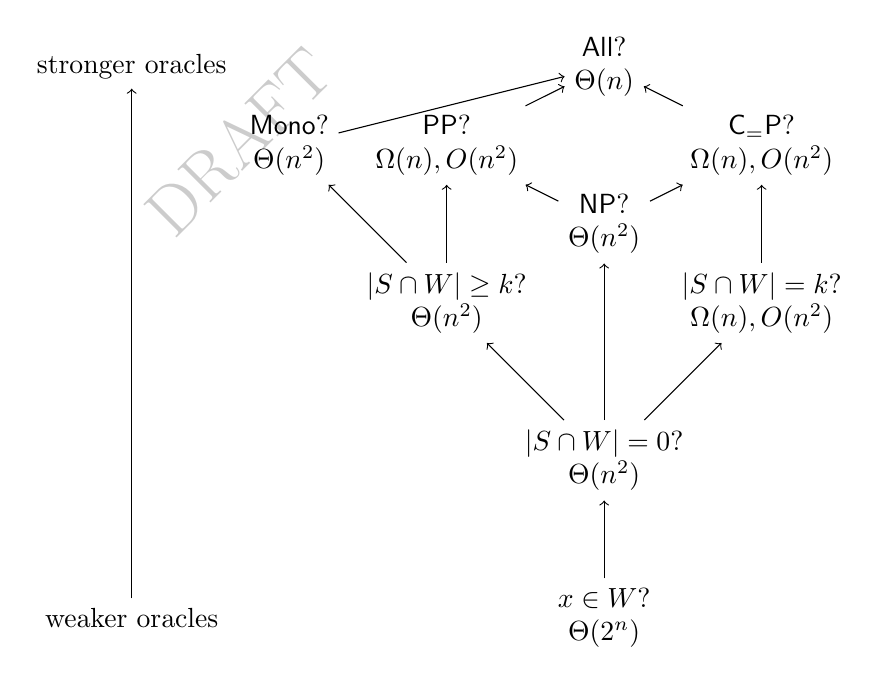
\begin{tikzpicture}[->, every node/.style={align=center}]
      \node at (0, 0) (direct) {$x \in W?$ \\ $\Theta(2^n)$};
      \node at (0, 2) (equal0) {$|S \cap W| = 0?$ \\ $\Theta(n^2)$};
      \node at (0, 5) (NP) {$\NP?$ \\ $\Theta(n^2)$};
      \node at (-2, 4) (geqk) {$|S \cap W| \geq k?$ \\ $\Theta(n^2)$};
      \node at (2, 4) (eqk) {$|S \cap W| = k?$ \\ $\Omega(n), O(n^2)$};
      \node at (-2, 6) (PP) {$\PP?$ \\ $\Omega(n), O(n^2)$};
      \node at (2, 6) (CeP) {$\CeP?$ \\ $\Omega(n), O(n^2)$};
      \node at (-4, 6) (mono) {$\mathsf{Mono}?$ \\ $\Theta(n^2)$};
      \node at (0, 7) (all) {$\mathsf{All}?$ \\ $\Theta(n)$};
      \draw (direct) to (equal0);
      \draw (equal0) to (NP);
      \draw (equal0) to (geqk);
      \draw (equal0) to (eqk);
      \draw (eqk) to (CeP);
      \draw (geqk) to (PP);
      \draw (geqk) to (mono);
      \draw (NP) to (CeP);
      \draw (NP) to (PP);
      \draw (PP) to (all);
      \draw (mono) to (all);
      \draw (CeP) to (all);

      \node at (-6, 0) (weak) {weaker oracles};
      \node at (-6, 7) (strong) {stronger oracles};
      \draw (weak) to (strong);
    \end{tikzpicture}
  \end{center}
\end{figure}

\section{Relationship among algorithms}

The equivalence of the $\NP$ and $\coNP$ oracles suggested in the previous section is given by a corollary to the following proposition.

\begin{proposition}\label{prop:flip}
  Suppose $W$ is a witness set and $k$ is positive integer.
  \begin{itemize}
  \item There is a witness-finding algorithm with intersection query oracle $A^{\geq k}_W$ if and only if there is a witness-finding algorithm with intersection query oracle $A^{< k}_W$.
  \item There is a witness-finding algorithm with intersection query oracle $A^{= k}_W$ if and only if there is a witness-finding algorithm with intersection query oracle $A^{\neq k}_W$.
  \end{itemize}
  Furthermore, in both cases, the seed length, success probability, and query complexity of the algorithms are exactly the same.
\end{proposition}
\begin{proof}
  For any query set $Q$, by definition we have
  \begin{equation*}
    \overline{A^{\geq k}_W(Q)} = A^{< k}_W(Q)
  \end{equation*}
  and
  \begin{equation*}
    \overline{A^{= k}_W(Q)} = A^{\neq k}_W(Q),
  \end{equation*}
  so if we define $\overline{\mc{F}}$ by
  \begin{equation*}
    \overline{\mc{F}}(s, A_1, \dotsc, A_m) = \mc{F}(s, \overline{A_1}, \dotsc, \overline{A_m}),
  \end{equation*}
  for all random seeds $s$ and all possible oracle answers $A_1, \dotsc, A_m$, we get the desired equivalence: $(\mc{Q}, \mc{F})$ is equivalent to $(\mc{Q}, \overline{\mc{F}})$.
\end{proof}

\begin{corollary}\label{cor:flip}
  Suppose $W$ is a witness set.
  There is a witness-finding algorithm with intersection query oracle $A^{= 0}_W$ if and only if there is a witness-finding algorithm with intersection query oracle $A^{\neq 0}_W$.
  Furthermore, the seed length, success probability, and query complexity of the algorithms are exactly the same.
\end{corollary}

\todo{This proposition uses two oracles instead of one...this isn't defined in our model.}

\begin{proposition}
  If there is a witness-finding algorithm with intersection query oracle $A^{=k}_W$ with query complexity $m$, then there is a witness-finding algorithm with access to two intersection query oracles, $A^{\geq k}_W$ and $A^{\geq k + 1}_W$,  with query complexity $2m$.
  Furthermore, the seed length and success probability of the algorithms are exactly the same.
\end{proposition}
\begin{proof}
  Suppose $(\mc{Q}, \mc{F})$ is the witness-finding algorithm with intersection query oracle $A^{=k}_W$.
  By \autoref{prop:flip}, it suffices to show a witness-finding algorithm with access to the two oracles $A^{\geq k}_W$ and $A^{< k + 1}_W$, or equivalently, $A^{\geq k}_W$ and $A^{\leq k}_W$.
  Define $\mc{Q}'$ by
  \begin{equation*}
    \mc{Q}'(s) = (Q_1, Q_2, \dotsc, Q_m, Q_1, \dotsc, Q_m),
  \end{equation*}
  where $(Q_1, \dotsc, Q_m)$ is the output of $\mc{Q}(s)$.
  Let $A^\geq_i$ and $A^\leq_i$ denote $A^{\geq k}_W(Q_i)$ and $A^{\geq k}_W(Q_i)$, respectively, for each $i \in [m]$.
  Define $\mc{F}'$ by
  \begin{equation*}
    \mc{F}'(s, A^\geq_1, \dotsc, A^\geq_m, A^\leq_1, \dotsc, A^\leq_m) = \mc{F}(s, A^\geq_1 \land A^\leq_1, \dotsc, A^\geq_m \land A^\leq_m).
  \end{equation*}
  Since $A^\geq_i \land A^\leq_i = A^{= k}_W(Q_i)$, the correctness of $(\mc{Q}', \mc{F}')$ follows from the correctness of $(\mc{Q}, \mc{F})$.
\end{proof}

The problem of finding a hitting algorithm reduces to the problem of finding an isolation query algorithm.

\begin{lemma}\label{lem:reduction}
  Suppose there is a (nonadaptive or adaptive) isolation query algorithm with success probability $p$ and query complexity $m$.
  Then there is a hitting algorithm with success probability $p$ and query complexity $m + 1$.
\end{lemma}
\begin{proof}
  Suppose $(\mc{Q}, \mc{F})$ is the isolation query algorithm.
  Construct hitting algorithm $\mc{P}$ with access to isolation oracle $A^{=1}_W$ as follows.
  \begin{itemize}
  \item simulate $\mc{Q}(s)$ to generate queries $Q_1, \dotsc, Q_m$ (simulating access to the isolation oracle if adaptivity is required)
  \item send those queries to the oracle $A^{=1}_W$ to get answers $A_1, \dotsc, A_m$
  \item simulate $\mc{F}(s, A_1, \dotsc, A_m)$ to output a string $w$.
  \item let $Q_{m + 1} = \{ w \}$ and output $Q_1, \dotsc, Q_{m + 1}$
  \end{itemize}

  Let $W$ be an arbitrary witness set and suppose the success probability of the isolation query algorithm $(\mc{Q}, \mc{F})$ is $p$.
  This is the probability that $w \in W$, or in other words, the probability that $|Q_{m + 1} \cap W| = 1$.
  Since $Q_{m + 1}$ is the last query set output by $\mc{P}$, the probability that $\mc{P}$ succeeds with respect to $W$ equals the probability that $(\mc{Q}, \mc{F})$ succeeds with respect to $W$.
  Thus $\mc{P}$ has success probability $p$ and query complexity $m + 1$.
\end{proof}

On the other hand, there does not seem to be a general reduction from an isolation query algorithm to a hitting algorithm.
In order to output a single witness knowing only that a witness is contained in a particular query set doesn't help, unless the query set is small; there is no such guarantee on the size of that set.

\begin{conjecture}
  Under an appropriate setting of parameters, if the existence of a hitting algorithm implies the existence of an isolation query algorithm, then $\RP = \NP$.
  \todo{As shown in the next section, both types of algorithms exist with the same parameters.}
\end{conjecture}

Now, consider the possibility that a witness-finding algorithm with intersection query oracle $A^{= k}_W$ implies an algorithm with oracle $A^{= k - 1}_W$.
Intuitively, in order for this to work, the latter algorithm would have to simulate the queries $Q_i$ from the former algorithm with some sort of collection of queries of the form $Q_i \setminus \{q_{i, j}\}$, where $q_{i, j}$ is the $j$th member of $Q_i$.
However, the oracle answers would be inconsistent, because we don't know beforehand whether $q_{i, j}$ is in the witness set or not (causing a discrepancy between the answers of the two oracles).
A similar problem arises when attempting the converse simulation: the simulated queries would be something of the form $Q_i \cup \{v_j\}$, where $v_j$ is the $j$th element of $\Sigma^n \setminus Q_i$, thus there would be a discrepancy between the answers of the two oracles.
We therefore conjecture that there is evidence that such a simulation is unlikely.

\begin{conjecture}
  For each $k \in \left[2^n\right]$, if the existence of a witness-finding algorithm with intersection query oracle $A^{= k}_W$ implies the existence of a witness-finding algorithm with intersection query oracle $A^{= k + 1}_W$, then $\RP = \NP$.
  \todo{But both $A^{= 0}_W$ and $A^{= 1}_W$ algorithms exist unconditionally, as shown in the next section.}
\end{conjecture}

\subsection{Reductions to counting classes}

In \autocite[Section~7]{green93}, Fred asks, ``Does the hypothesis $\P^{\CeP} = \P^\PP$ have any dramatic consequences?''
Our intuition is that $\P^{\CeP}$ is less powerful than $\P^\PP$, because the latter can determine the exact number of accepting paths in a computation (or in other words, the number of witnesses in a witness set) by a binary search, whereas the former does not seem to admit this possibility.
On the contrary, we know that $\NP^{\CeP} = \NP^\PP$.
Perhaps a first step toward comparing $\P^\PP$ and $\P^{\CeP}$ is comparing $\RP^\PP$ and $\RP^{\CeP}$.

There is a superficial similarity to the question ``is $\RP^\PP$ a subset of $\RP^{\CeP}$?'' and the question ``does a witness-finding algorithm with oracle $A^{\geq k}_W$ imply a witness-finding algorithm with oracle $A^{= k}_W$?''
However, we run into a few problems when trying to follow this approach.
First, according to \autocite[Remark~2]{krw12}, the lower bounds on emptiness query algorithms (with oracle $A^{=0}_W$) ``essentially hold'' when the oracle is $A^{\geq k}_W$ instead, for any $k$ bounded by a polynomial in $n$.
Furthermore, if we attempt such a proof, we run into several problems.

\begin{conjecture}
  If $\RP^\PP \subseteq \RP^{\CeP}$, then a witness-finding algorithm with oracle $A^{\geq k}_W$ implies a witness-finding algorithm with oracle $A^{= k}_W$.
\end{conjecture}
\begin{proof}[Broken proof]
  Let $W$ be any witness set.
  Let $(\mc{Q}, \mc{F})$ be a witness-finding algorithm with oracle $A^{= k}_W$.
  Let $L$ be a witnessed language with witness relation $L'$.
  The problem of deciding whether $|Q \cap W| \geq k$ given any query set $Q$ can be decided by a $\PP$ oracle.
  Construct machine $M$ with access to that oracle as follows on random string $s$ of length $r$.
  \begin{itemize}
  \item Run $\mc{Q}(s)$ to generate queries $Q_1, \dotsc, Q_m$, simulating access to the $\PP$ oracle (acting as the $A^{\geq k}_W$ oracle) when necessary.
  \item Get query answers $A_1, \dotsc, A_m$ from the oracle.
  \item Run $\mc{F}(s, A_1, \dotsc, A_m)$ to get potential witness $w$.
  \item Decide if $(x, w) \in L'$.
  \end{itemize}
  \todo{Problem 1: need to show that this is a correct $\RP^\PP$ algorithm.}
  By our hypothesis that $\RP^\PP \subseteq \RP^{\CeP}$, there is also a randomized oracle machine $M'$ that decides $L$ with access to a $\CeP$ oracle.
  Now we wish to use $M'$ to construct a witness-finding algorithm $(\mc{Q}', \mc{F}')$ with access to oracle $A^{= k}_W$.

  Define $\mc{Q}'$ as follows on random string $s$ of length $r$.
  \begin{itemize}
  \item Run $M'(x, s)$ and intercept each query $q_1, \dotsc, q_{m(n)}$ that it would make to the $\CeP$ oracle.
    \todo{Problem 2: $M'$ needs access to a particular input string $x$; we may be able to modify the definition of the witness-finding algorithms to allow this.}
    Each query $q_i$ is a question of the form ``is $|W_{q_i}| = k$?'', where $W_{q_i}$ is a witness set that corresponds to the input string $q_i$, so we simulate those queries by sending the query set $W_{q_i}$ to the oracle $A^{= k}_W$.
    \todo{Problem 3: this won't work, since $A^{= k}_W$ only answers questions of the form ``is $|W_{q_i} \cap W| = k$?'', but we need it to answer questions like ``is $|W_{q_i}| = k$?'', and we don't get to choose the arbitrary witness set $W$.}
  \item Output the queries $W_{q_1}, \dotsc, W_{q_{m(n)}}$.
  \end{itemize}
  Define $\mc{F}'$ as follows on random string $s$ and oracle answers $A_1, \dotsc, A_{m(n)}$.
  \begin{itemize}
  \item Run $M'(x, s)$ and when $M'$ makes query $q_i$, provide answer $A_i$ to it.
  \item \todo{Problem 4: at this point, all $M'$ tells us is that there is a witness (or none); it gives no indication as to what the witness is.
    If one of the queries causes the oracle to answer yes and the size of the query set is not too large, we could simply output a random element of the query set for a small penalty in success probability, but in general we have no such guarantees.}
  \end{itemize}
\end{proof}

Although this starts to have little to do with the witness-finding algorithm results given in the following sections, another approach to showing that $\P^{\CeP} \neq \P^\PP$ may be to show that adaptive queries to $\CeP$ are no more powerful than nonadaptive queries, whereas adaptive queries to $\PP$ are more powerful than adaptive queries.
What is known about $\PP$?
\begin{itemize}
\item $\PP$ is closed under complement, union, and intersection.
\item $\PP = \P^{\PP[O(1)]}_\parallel$ (that is, $\PP$ is closed under polynomial time $k$-round truth-table reductions, for any $k \in O(1)$).
\end{itemize}
What is known about $\CeP$?
\begin{itemize}
\item $\P^{\CeP[O(1)]}_\parallel = \P^{\CeP[O(\log n)]}$ (see \autocite[Theorem~5]{green93} and \autocite[Corollary~4.6]{ogiwara94}).
\end{itemize}

\section{Upper bounds}

\begin{theorem}\label{thm:naive}
  There is a polynomial time adaptive emptiness query algorithm with success probability $1$ and query complexity $O(n)$.
\end{theorem}
\begin{proof}[Proof idea]
  By \autoref{cor:flip}, it suffices to show a $A_W^{\neq 0}$ witness-finding algorithm.
  This the well-known bit-by-bit $\P^\NP$ computable function for computing a witness for a given string.

  For each $i \in [n]$ and each $b \in \{0, 1\}$, define the query $Q_{i, b}$ inductively (or in other words, adaptively) as follows.
  If $i = 1$, then $Q_{i, b} = \{ b v \, | \, v \in {\{0, 1\}}^{n - 1}\}$.
  For each subsequent pair of queries, let $u = b_1 \dotsb b_{i - 1}$, where $b_j$ is a bit that caused the oracle to answer ``yes'' on query $Q_{j, b_j}$ for each $j \in [i - 1]$, and let $Q_{i, b} = \{ u b v \, | \, v \in {\{0, 1\}}^{n - i}\}$.
  Finally, given the responses to $Q_{n, 0}$ and $Q_{n, 1}$, which are singleton sets, the algorithm simply outputs the sole element of the query set that caused the oracle to answer ``yes''.

  The total number of queries is $2n$, which is in $O(n)$.
\end{proof}

\begin{theorem}[{\autocite[Proposition~1]{krw12} (citing \autocite{bcgl92})}]
  There is a polynomial time nonadaptive emptiness query algorithm with success probability $\Omega(1)$ and query complexity $O(n^2)$.
\end{theorem}
\begin{proof}[Proof idea]
  By \autoref{cor:flip}, it suffices to show a $A_W^{\neq 0}$ witness-finding algorithm.
  This algorithm uses the Valiant--Vazirani Isolation Lemma in each query to guess each bit of a possible witness (in parallel).

  First, consider a simpler set of queries.
  Let $s$ be a string in $\Sigma^r$.
  For each $i \in [n]$ and each $b \in \Sigma$, let $Q_{i, b} = \{ w \, | \, w \in C_s \land w_i = b\}$, where $C$ is the isolating set from the Valiant--Vazirani Isolation Lemma (for example, the set of all strings whose image is zero under a pairwise independent hash function).
  The Valiant--Vazirani Isolation Lemma proves that this algorithm has success probability $\Omega(\frac{1}{n})$ and query complexity $O(n)$.
  In order to get success probability $\Omega(1)$, we create $O(n)$ collections of $O(n)$ queries, with an independent set $C_{s_k}$ for each collection.
  Now our queries are $Q_{k, i, b} = \{ w \, | \, w \in C_{s_k} \land w_i = b\}$, for each $k \in \left[O(n)\right]$, each $i$, and each $b$.
\end{proof}

In \autocite{krw12}, the authors call the above theorem the ``truth-table reduction'' analog of the ``many-one reduction'' result of \autocite[Theorem~4.2]{dkvmw13}.
However, this is not strictly precise, since the former involves an emptiness oracle, whereas the latter involves an isolation oracle.
Fortunately, the proof uses the Valiant--Vazirani Isolation Lemma (that is, the sets $C_{s_k}$), so the probability that $|Q \cap W| \neq 0$ equals the probability that $|Q \cap W| = 1$.

\begin{corollary}
  There is a polynomial time nonadaptive isolation query algorithm with success probability $\Omega(1)$ and query complexity $O(n^2)$.
\end{corollary}

\todo{Double check this logic.}

\begin{corollary}
  There is a polynomial time hitting algorithm with success probability $\Omega(1)$ and query complexity $O(n^2)$.
\end{corollary}
\begin{proof}
  Combine the previous corollary with \autoref{lem:reduction}.
\end{proof}

\section{Lower bounds}

\begin{theorem}[{\autocite[Theorem~2]{krw12}}]\label{thm:nonadaptiveemptiness}
  For any nonadaptive emptiness query algorithm, if the algorithm has success probability $\Omega(1)$, then it has query complexity $\Omega(n^2)$.
\end{theorem}

The proof of this theorem relies on the existence of a distribution on witness sets that places all witnesses far apart, so it is hard to guess both the number and location of the witnesses.
This distribution comes from \autocite[Theorem~4.2]{dkvmw13}.

\begin{corollary}[{\autocite[Remark~2]{krw12}}]
  Let $p$ be a polynomial.
  For any nonadaptive $A^{\geq p(n)}_W$ witness-finding algorithm, if the algorithm has success probability $\Omega(1)$, then it has query complexity $\Omega(n^2)$.
\end{corollary}

\begin{theorem}[{\autocite[Theorems~3.3 and 3.4]{newport14}}]
  For any hitting algorithm, if the algorithm has success probability $\Omega(1 - 2^{-n})$, then it has query complexity $\Omega(n^2)$.
  Furthermore, this is true even when restricted to witness sets of cardinality two.
\end{theorem}

The proof of this theorem relies on the probabilistic method to show the existence of a witness set that is hard to ``hit'', found in \autocite{ablp91}.

\begin{corollary}\label{cor:isolationalg}
  For any adaptive isolation query algorithm, if the algorithm has success probability $\Omega(1 - 2^{-n})$, then it has query complexity $\Omega(n^2)$.
  Furthermore, this is true even when restricted to witness sets of cardinality two.
\end{corollary}
\begin{proof}
  This is a proof by contradiction.
  Assume there is an adaptive isolation algorithm with success probability $\Omega(1 - 2^{-n})$ and query complexity $o(n^2)$.
  By \autoref{lem:reduction}, there is a hitting algorithm with the same success probability and query complexity (up to constant factors).
  This would contradict the previous theorem, hence no such algorithm exists.
\end{proof}

This corollary is similar to \autoref{thm:nonadaptiveemptiness}, but is stronger in some ways and weaker in others.
It is stronger in two ways.
First, not only nonadaptive algorithms but also adaptive algorithms have this lower bound.
Second, its isolation query oracle is like a $\US$ oracle, more powerful than the emptiness query oracle, which is like an $\NP$ oracle.
However, it is weaker in that it requires the success probability to be $\Omega(1 - 2^{-n})$, asymptotically much greater than $\Omega(1)$.

Other types of queries produce the same lower bounds.
Queries of the form ``does $|Q \cap W| = |Q|$?'', or equivalently, ``is $Q \subseteq W$?'', yield the same lower bounds as in \autoref{thm:nonadaptiveemptiness}.
Such queries are \emph{monotone queries} (that is, if $W \subseteq W'$, then $Q \subseteq W$ implies $Q \subseteq W'$), and monotone queries with constant success probability have $o(n^2)$ query complexity \autocite[Theorem~1.3]{krw14}.

\begin{theorem}[{\autocite[Theorem~3.2]{newport14}}]
  There is no hitting algorithm with (expected success probability ??? and) expected query complexity $o(n)$.
\end{theorem}

\todo{I can't understand what the random variable is for which there is an expectation here.}

\section{Entropy on bad witness distributions}

In this section $H(X)$ denotes the Shannon entropy of random variable $X$ chosen from a distribution on binary strings, and $H_b(p)$ denotes the binary entropy function on a Bernoulli process with success probability $p$.

Define $\mc{W}_n^*$, a distribution on witness sets (that is, subsets of $\Sigma^n$), by the following sampling procedure.
\begin{itemize}
\item Let $W = \emptyset$.
\item Choose $D$ uniformly at random from $[n]$.
\item For each $w \in \Sigma^n$, add $w$ to $W$ with probability $2^{-D}$.
\item Output $W$.
\end{itemize}
(Technically, $W$ may be the empty set, but this occurs with probability $o(1)$, so for our purposes, we ignore it.
\todo{a brief explanation can be found in \autocite{krw14}, I believe.})

\begin{lemma}\label{lem:prob}
  For any positive integer $n$, for any $k \in [2^n]$, for any $d \in [n]$, and for any $S \subseteq \left(\left\{0, 1\right\}^n \setminus \emptyset\right)$,
  \begin{equation*}
    \Pr_{W \gets \mc{W}_n^*}\left[ |S \cap W| = k \middle| D = d\right] < \frac{e^{\frac{1}{12s}}}{\sqrt{2 \pi}} \left(\frac{s}{k (s - k)}\right)^{\frac{1}{2}},
  \end{equation*}
  where $s$ denotes the cardinality of $S$.
\end{lemma}
\begin{proof}
  For the sake of brevity, let $s$ denote $|S|$, and let $p$ denote the probability $\Pr_{W \gets \mc{W}_n^*}[ |S \cap W| = k | D = d]$.
  Without loss of generality, assume $s \geq k$, since if $s$ is smaller than $k$, the probability $p$ is zero.
  Since each element in $W$ is chosen independently with probability $2^{-d}$, the probability that $|S \cap W| = k$ is the probability that exactly $k$ of the elements of $S$ are in $W$ and exactly $s - k$ of the elements are not in $W$.
  This probability fits the binomial distribution with $s$ trials, $k$ successes, and probability of success $2^{-d}$.
  Thus
  \begin{equation*}
    p = \binom{s}{k} (2^{-d})^k (1 - 2^{-d})^{s - k}.
  \end{equation*}
  By finding the zeros of the first derivative of $p$ with respect to $d$, we see that $p$ achieves a maximum value at $d = -\log \frac{k}{s}$.
  \todo{Cite a text giving the first derivative of the binomial distribution.}
  When $d$ takes this value,
  \begin{equation*}
    p = \binom{s}{k} \frac{k^k}{s^s} (s - k)^{s - k}.  % so fun!
  \end{equation*}
  Expanding the binomial coefficient as $\frac{s!}{k!(s - k)!}$ and applying Stirling's approximation,
  \begin{equation*}
    \sqrt{2 \pi m} \left(\frac{m}{e}\right)^m < m! < e^{\frac{1}{12m}} \sqrt{2 \pi m} \left(\frac{m}{e}\right)^m,
  \end{equation*}
  yields the upper bound
  \begin{equation*}
    %p & < \frac{\sqrt{2 \pi s} \left(\frac{s}{e}\right)^s e^{\frac{1}{12s}} k^k (s - k)^{s - k}}{\sqrt{2 \pi (s - k)} \left(\frac{s - k}{e}\right)^{s - k} e^{\frac{1}{12 (s - k) + 1}} \sqrt{2 \pi k} \left(\frac{k}{e}\right)^k e^{\frac{1}{12 k + 1}}} \\
    %p & < \frac{\sqrt{2 \pi s} \left(\frac{s}{e}\right)^s e^{\frac{1}{12s}} k^k (s - k)^{s - k}}{\sqrt{2 \pi (s - k)} \left(\frac{s - k}{e}\right)^{s - k} \sqrt{2 \pi k} \left(\frac{k}{e}\right)^k} \\
    p < \frac{e^{\frac{1}{12s}}}{\sqrt{2 \pi}} \left(\frac{s}{k (s - k)}\right)^{\frac{1}{2}}. \qedhere
  \end{equation*}
  %\todo{See \url{http://faculty.cs.tamu.edu/klappi/random-s06/useful_bounds.pdf} for better bounds, perhaps.}
\end{proof}

Under what relationship between $k$ and $|S|$ does the probability become at most one half?

\begin{lemma}\label{lem:quad}
  Let $n$, $k$, $d$, $S$, and $s$ be as in the hypothesis of \autoref{lem:prob}.
  If $s \geq 4$ and $k$ satisfies either of the inequalities
  \begin{equation*}
    k \leq \frac{1}{2}\left(s - \frac{1}{\alpha} \sqrt{s (s - 4)}\right)
  \end{equation*}
  or
  \begin{equation*}
    k \geq \frac{1}{2}\left(s + \frac{1}{\alpha} \sqrt{s (s - 4)}\right),
  \end{equation*}
  where $\alpha = \frac{20}{103}$, then
  \begin{equation*}
    \frac{e^{\frac{1}{12s}}}{\sqrt{2 \pi}} \left(\frac{s}{k (s - k)}\right)^{\frac{1}{2}} \leq \frac{1}{2}.
  \end{equation*}
\end{lemma}
\begin{proof}
  Since $s \geq 4$, we have $\frac{1}{12 s} \leq \frac{1}{48}$, so $e^\frac{1}{12 s} \leq e^{\frac{1}{48}} \leq 1.03$.
  Also, the value of $\frac{1}{\sqrt{2 \pi}}$ is less than $0.4$.
  Thus it suffices to show that
  \begin{equation*}
    \frac{1.03}{0.4} \left(\frac{s}{k (s - k)}\right)^{\frac{1}{2}} \leq \frac{1}{2},
  \end{equation*}
  or equivalently,
  \begin{equation*}
    \frac{s}{k (s - k)} \leq \left(\frac{20}{103}\right)^2 = \alpha^2.
  \end{equation*}

  We can rearrange this inequality so that it looks like the more familiar quadratic inequality in the variable $k$,
  \begin{equation*}
    -\alpha^2 k^2 + \alpha^2 k s - s \geq 0.
  \end{equation*}
  The discriminant of this quadratic polynomial is $\alpha^2 s^2 - 4(-\alpha^2)(-s)$, which equals $\alpha^2 s (s - 4)$.
  Since $s \geq 4$ by hypothesis, the polynomial has real roots.
  Since this polynomial is convex, the inequality is satisfied when $k$ lies outside the open interval whose endpoints are the two (possibly equal) roots.
  The quadratic formula proves that the roots of the polynomial are
  \begin{equation*}
    \frac{s}{2} \pm \frac{1}{2 \alpha^2} \sqrt{\alpha^2 s (s - 4)}.
  \end{equation*}
  We conclude that the upper bound in the conclusion of the lemma is satisfied if $k$ is outside the interval
  \begin{equation*}
    \left(\frac{1}{2}\left(s - \frac{1}{\alpha} \sqrt{s (s - 4)}\right), \frac{1}{2}\left(s + \frac{1}{\alpha} \sqrt{s (s - 4)}\right)\right). \qedhere
  \end{equation*}
\end{proof}

If the probability of a Bernoulli trial is less than one half, this provides an upper bound on the binary entropy of the probability.

\begin{lemma}
  Let $n$, $k$, $d$, $S$, and $s$ be as in the hypothesis of \autoref{lem:quad}.
  Suppose $W \gets \mc{W}^*_n$ and let $A$ denote the Bernoulli random variable for the event $|S \cap W| = 1$, conditioned on the event $D = d$.
  We have
  \begin{equation*}
    H_b(A) \leq -2 \frac{e^{\frac{1}{12s}}}{\sqrt{2 \pi}} \left(\frac{s}{k (s - k)}\right)^{\frac{1}{2}} \log \left(\frac{e^{\frac{1}{12s}}}{\sqrt{2 \pi}} \left(\frac{s}{k (s - k)}\right)^{\frac{1}{2}}\right).
  \end{equation*}
\end{lemma}
\begin{proof}
  If $p$ is at most $q$ and $q \leq \frac{1}{2}$, then $H_b(p) \leq -2 q \log q$.
  Apply this fact with the previous two lemmas, choosing $q$ to be $\frac{e^{\frac{1}{12s}}}{\sqrt{2 \pi}} \left(\frac{s}{k (s - k)}\right)^{\frac{1}{2}}$.
\end{proof}

\begin{lemma}
  Let $n$, $d$, $S$, and $s$ be as in the hypothesis of the previous lemma.
  For any $k \in [2^n]$, if
  \begin{equation*}
    p^{= k} = \Pr_{W \gets \mc{W}_n^*}[ |S \cap W| = k | D = d]
  \end{equation*}
  and
  \begin{equation*}
    p^{\geq k} = \Pr_{W \gets \mc{W}_n^*}[ |S \cap W| \geq k | D = d],
  \end{equation*}
  then
  \begin{equation*}
    p^{\geq k} = \sum_{i = k}^{s} p^{= i}.
  \end{equation*}
\end{lemma}
\begin{proof}
  The first equality holds because
  \begin{align*}
    p^{\geq k} & = \Pr_{W \gets \mc{W}_n^*}\left[ |S \cap W| \geq k \middle| D = d \right] \\
    & = \Pr_{W \gets \mc{W}_n^*}\left[ \bigcup_{i = k}^{s} |S \cap W| = i \middle| D = d \right] \\
    & = \sum_{i = k}^{s} \Pr_{W \gets \mc{W}_n^*}\left[ |S \cap W| = i \middle| D = d\right] \\
    & = \sum_{i = k}^{s} p^{= i},
  \end{align*}
  where the third equality holds because the events $|S \cap W| = i$ and $|S \cap W| = j$ are mutually exclusive for any distinct $i$ and $j$ in $[2^n]$.
\end{proof}

\section{Todo}

Does the lower bound of \autoref{cor:isolationalg} hold for any algorithm asking queries to an oracle that answers questions of the form ``does $|Q \cap W| = k$?'' for any fixed positive integer $k$?
(It certainly doesn't hold when $k = 0$, because of \autoref{thm:naive}.)
This question may be answered by adapting the proof by probabilistic method given in \autocite{ablp91}.
In \autocite[Remark~2]{krw12}, the authors state without proof that the lower bound in \autoref{thm:nonadaptiveemptiness} holds even for queries of the form ``is $|Q \cap W| > k$?'' (remember, they were originally considering not emptiness queries but \emph{nonemptiness} queries).

\printbibliography{}

\end{document}
